In the initial docking stage of the IDSITE protocol Glide is used to generate a number of proposed docked conformations for each ligand.
Glide (standard precision) is used to generate a number of different ligand conformations by sampling conformations of freely rotatable bonds and rings.
A bounding box, which will be used for a grid search, is defined centered at the centroid of the ligand with an edge length of 10 angstroms.
Because the crystal structure used for CYP2D6 (PDBID: 2F9Q) does not have a ligand, the centroid of residues Glu216, Asp301, Thr309, and Phe483 was used instead in this case.
Because the steric clashes present in many proposed docked conformations can be relieved using a simple minimization procedure a reduced Van der Waals (VDW) radii are used in the docking stage for non-polar atoms.
The VDW radii used for the P450 are scaled by a factor of 0.4, and the scaling for the ligand starts at 0.8.
If an insufficient number of poses, in this case fewer than four, are found using these scaling factors for the radii the scaling of the ligand is stepped down until at least four poses are found.
Additional filtering of possible high energy conformations was also skipped in order to ensure the greatest diversity of docked poses reached the refinement stage.
The collection of docked poses are then clustered according to the RMSD of the ligand, and each pose is minimized.
The top sixty ranked poses according to the Glide SP metric are retained screened using a number of different criteria.
A hard sphere overlap criteria is used to remove poses with obvious steric clashes which were not removed during the minimization procedure.
A conserved feature of CYP2D6 ligand complexes is a salt bridge with Glu216 or Asp301.
In order to reduce sampling cost IDSITE only considers structures with at least one hydrogen-bond donor within 4 residues of the centroid of these two residues and Ser304.
The sphere defined by these residues is illustrated along with the bounding box used for sampling in Figure \ref{fig:idsite_glide}
A number of other rule based geometric screens are used to remove structures which are unlikely to react.
Structures where:
\begin{enumerate}
\item The distance of the basic nitrogen to the ferryl oxygen is less than 5.0 angstroms;
\item The distance of the basic nitrogen to the negative charged oxygen (in Glu216 or Asp301) is greater than 5.5 angstroms;
\item More than 2 heavy atoms from the ligands are further than 16.0 angstroms away from the heme iron;
\item More than 1 heavy atom from the ligand are closer than 1.0 angstroms to the receptor;
\item More than 6 heavy atoms from the ligand are closer than 1.8 angstroms to the receptor;
\item No heavy atom in the ligand is within 5.0 angstroms to the heme iron;
\end{enumerate}
are removed and the remaining poses are passed on to the first Monte Carlo Minimization refinement stage.

\begin{figure}[h]
\centering
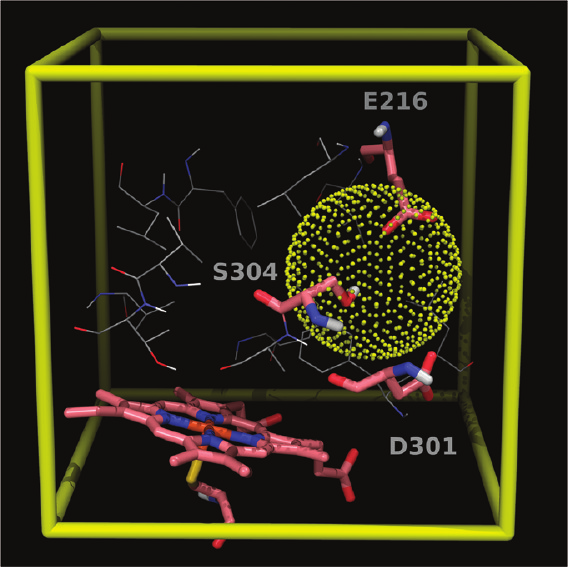
\includegraphics[width=0.35\textwidth]{figures/idsite/glide.png}
\caption{An overview of the entire IDSite procedure.}
\label{fig:idsite_glide}
\end{figure}

% IDSite uses reduced VDW radii for nonpolar atoms both in the protein receptor and the ligand, so that slight steric clashes are tolerated during the docking stage.
% For the protein receptor the VDW scaling factor is fixed at 0.40, while for the ligand, the scaling factor starting from 0.80 is adaptively adjusted until at least 4 valid poses are found.
% With highly flexible ligands and relatively high scaling factors, Glide often finds only a handful of valid poses, and even fewer survive after IDSite screening.
% However, if the scaling factor is set too low, the docked poses may contain too many serious steric clashes, which can cause problems in the subsequent minimization.
% If IDSite fails to find enough valid poses, the scaling factor is adjusted and the number of poses to pass the initial docking phase in Glide is increased accordingly to augment sampling.

% joe is this far
% If the ligand contains other hydrogen-bond donors except for the basic nitrogen, the constrained docking is likely to generate poses that form hydrogen bonds instead of the salt bridge to Glu216 or Asp301.
% However, IDSite is able to distinguish these poses and filter them via an additional salt bridge filter in the pose screening, so that only the poses with a stable salt bridge are allowed to pass to the refinement stage.
